\documentclass{article}

\usepackage{float}
\usepackage[utf8]{inputenc}
\usepackage{hyperref}
%\usepackage[hyperref=true, natbib=true, style=numeric, backend=bibtex]{biblatex}
\usepackage{graphicx}
%\bibliography{references.bib}

\title{TCP Congestion Algorithms In Datacenters \\
	\vspace{0.3cm}
	{\large LS Project}
}
\date{\today{}}
\author{Luc Gommans, Rick van Gorp}

\begin{document}
\maketitle

\section{Abstract}


\section{Introduction}

% Copied from proposal

Multitentant datacenters aim to provide services with consistent performance
and reliability. When customers send a lot of data in a short amount of time,
networks might become congested, which results in lowered performance.

Congestion occurs when a buffer on the path to the recipient is full and
packets are dropped. TCP has a mechanism to avoid congestion in the network:
TCP congestion control. Multiple algorithms are available for congestion
control and show a different behaviour depending on the network's
characteristics.

In 2010, the algorithm DCTCP was described in an
article\cite{dctcp-congestion-original} and published as RFC8257 in
2017\cite{dctcp-congestion}. DCTCP is optimized for datacenters and provides a
high-burst tolerance, low latency, and high throughput when the datacenter has
a small part of the buffer available\cite{dctcp-congestion}. In 2016 another
algorithm was proposed: BBR. This is a TCP congestion algorithm created by
Google, which achieves higher bandwidths and lower latencies compared to other
TCP congestion methods\cite{bbr-congestion}. A comparison of BBR with
CUBIC\cite{bbr-congestion-comparison} shows that the BBR node pushes the CUBIC
node away in bandwidth when using small buffers. The BBR node gets more
bandwidth allocated than the CUBIC node.

We propose to do a performance and behaviour analysis of different TCP
congestion control algorithms in a (simulated) datacenter network. Based on the
results, we will recommend datacenters on measures to keep providing a reliable
environment for customers when multiple congestion control algorithms are
active in the network, for example by using QoS or discouraging certain
congestion control algorithms.


\section{Related work}

% Copied from proposal

The TCP congestion control algorithm BBR is discussed in \cite{bbr-congestion}.
The journal contains a performance test of the BBR algorithm and a comparison
between the BBR algorithm and the CUBIC algorithm, where a noticeable
difference in bandwidth allocation is shown when using small buffers.

In \cite{multiple-congestion} a performance analysis of multiple TCP congestion
control algorithms is performed. This research does not include the new
congestion control algorithms we want to analyze and does not include the
datacenter context.

In \cite{dctcp-congestion-original} an algorithm is proposed to avoid
congestion within datacenters. The authors describe an algorithm that maintains
a small buffer occupancy and has an early detection of congestion.


\section{Method}
During this research a performance test of various TCP congestion algorithms will be performed. The TCP congestion algorithms will be determined through desk research of the most common algorithms. The tests will be conducted in a private environment. Based on the results of those tests, recommendations will be given related to the measures a datacenter has to take to keep the traffic equally allocated over customers. 
	
	\subsection{Comparing Performance}
	Two scenarios will be used to compare the performance of the TCP congestion algorithms:
	\begin{enumerate}
		\item The user owns one endpoint in the network. In this case only the sender side has a congestion algorithm applied.
		\item The user owns multiple endpoints in the network. In this case a congestion algorithm is applied at both the client and server side.
	\end{enumerate}
	
	The created environments are shown in figure ... and figure ...
	\begin{figure}[H] 
		\label{fig:setup1}
		\caption{Test setup: Scenario 1}
		\begin{center}
  			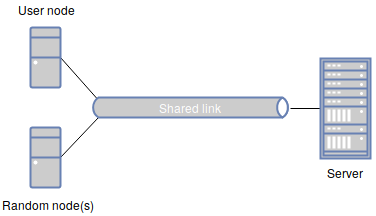
\includegraphics[scale=0.5]{figs/setup1.png}
  		\end{center}
	\end{figure}
	
\section{Results}


\section{Discussion}


\section{Conclusion}

% For reference, from the proposal:

Our main research question is:
{\it How can a datacenter provide an reliable and performant environment for
customers when multiple TCP congestion control algorithms are used in the
network?}

\vspace{0.5cm}

This main research question divides in five sub-questions:

\begin{enumerate}
	\item What TCP congestion algorithms are most commonly implemented in datacenter environments?
	\item How do these TCP congestion algorithms work?
	\item How do these TCP congestion algorithms differ in behavior?
	\item What is the impact on the availability and service for customers when using different, competing congestion algorithms?
	\item What measures could be taken to split bandwidth equally among tenants?
\end{enumerate}


%\printbibliography

\end{document}

